%Copyright 2019 Christopher M. Jermaine (cmj4@rice.edu) and Risa B. Myers (rbm2@rice.edu)
%
%Licensed under the Apache License, Version 2.0 (the "License");
%you may not use this file except in compliance with the License.
%You may obtain a copy of the License at
%
%    https://www.apache.org/licenses/LICENSE-2.0
%
%Unless required by applicable law or agreed to in writing, software
%distributed under the License is distributed on an "AS IS" BASIS,
%WITHOUT WARRANTIES OR CONDITIONS OF ANY KIND, either express or implied.
%See the License for the specific language governing permissions and
%limitations under the License.
%===============================================================
\documentclass[aspectratio=169]{beamer}
\mode<presentation> %use <handout> for handout mode
{
\usetheme[noshadow, minimal,numbers,riceb,nonav]{Rice}
\usefonttheme[onlymath]{serif}
\setbeamercovered{transparent}
}
\useinnertheme{rectangles}

\usepackage[english]{babel}

\usepackage{amsmath}
\usepackage{mathptmx}
\usepackage{helvet}
\usepackage{courier}
\usepackage[T1]{fontenc}
\usepackage{trajan}
\usepackage{ textcomp }
\renewcommand{\footnotesize}{\tiny}


\usepackage{listings}

\newenvironment{noindentitemize}
{ \begin{itemize}
 \setlength{\itemsep}{1.5ex}
  \setlength{\parsep}{0pt}   
  \setlength{\parskip}{0pt}
 \addtolength{\leftskip}{-2em}
 }
{ \end{itemize} }

\newenvironment{noindentitemize2}
{ \begin{itemize}
  \setlength{\itemsep}{0ex}
  \setlength{\parskip}{0pt}
  \setlength{\parsep}{0pt}   
  \addtolength{\leftskip}{-2em}  }
{ \end{itemize} }

\lstnewenvironment{SQL}
  {\lstset{
        aboveskip=5pt,
        belowskip=5pt,
        escapechar=!,
        mathescape=true,
        upquote=true,
        language=C,
        basicstyle=\linespread{0.94}\ttfamily\normalsize,
        deletekeywords={VALUE, PRIOR},
        showstringspaces=true}
        \vspace{0pt}%
        \noindent\minipage{0.47\textwidth}}
  {\endminipage\vspace{0pt}}
  
\newcommand{\LIKES}{\textrm{LIKES}} 
\newcommand{\FREQUENTS}{\textrm{FREQUENTS}} 
\newcommand{\SERVES}{\textrm{SERVES}} 
\newcommand{\CAFE}{\textrm{CAFE}} 
\newcommand{\COFFEE}{\textrm{COFFEE}} 
\newcommand{\DRINKER}{\textrm{DRINKER}} 
\newcommand{\ALLPEEPS}{\textrm{ALLPEEPS}} 
\newcommand{\ALLCOMBOS}{\textrm{ALLCOMBOS}} 

\setbeamerfont{block body}{size=\tiny}

%===============================================================%

\title[]
{Tools \& Models for Data Science}

\subtitle{Dimensionality Reduction}

\author[]{Chris Jermaine \& Risa Myers}
\institute
{
  Rice University 
}

\date[]{}

\subject{Beamer}

\begin{document}

\begin{frame}
 \titlepage
\end{frame}
%%***********************************************************
%\begin{frame}{Today's Topics}
%\begin{itemize}
%\item Not classification
%\item Not regression
%\item Dimensionality reduction
%\end{itemize}
%
%\begin{enumerate}
%	\item Eigenvalue / Eigenvector review
%	\item Sample data
%	\item The curse of dimensionality
%	\item 
%\end{enumerate}
%	
%\end{frame}
%***********************************************************
\begin{frame}{Our Scenario}

\begin{itemize}
\item We have high dimensional data and we want to make predictions on the data
\item ... or we want to classify the data
\item but, there's too much data
\item[?] What can we do?
\item Note: This is a ``What'' topic, not a ``How'' topic
% two approaches - fit to a probability distribution or Linear Regression
\end{itemize}
\end{frame}
%***********************************************************
\begin{frame}{Too much Data Problem}

\begin{itemize}
\item[?] What can we do?
\end{itemize}
\begin{enumerate}
\item We can use an approach that randomly samples from the data
\item[] ... not today
\item We can throw away data points % kind of the same as the prior point
\item[] ... that's almost always a bad idea
\item We can throw away features
\item[] ... let's explore this option
\end{enumerate}
\end{frame}
%***********************************************************
\begin{frame}{High Dimension Data}
\begin{itemize}
	\item What do we mean by ``high dimension''?
	\begin{itemize}
	\item Many, many features
	\item Can be millions!
	\item Lots of useless features obscure useful ones
	\item Example: Genomic data
	\begin{itemize}
	\item Comparing genome sequences
	\item Classifying genomes
	\end{itemize}
	\end{itemize}
\end{itemize}
	
\end{frame}

%***********************************************************
\begin{frame}{The Curse of Dimensionality}

%\begin{columns}
%\begin{column}{0.5\textwidth}

\begin{itemize}
		\item "As the number of features or dimensions grows, the amount of data we need to generalize accurately grows exponentially."
\begin{itemize}

	\item Charles Isbell, Professor and Senior Associate Dean, School of Interactive Computing, Georgia Tech
\end{itemize}
		\item Data become sparse in high dimensions
		\item All points are basically the same distance from one another
%		\item e.g. kNN doesn't work here with Euclidean distance
\end{itemize}
%\end{column}
%\begin{column}{0.5\textwidth}
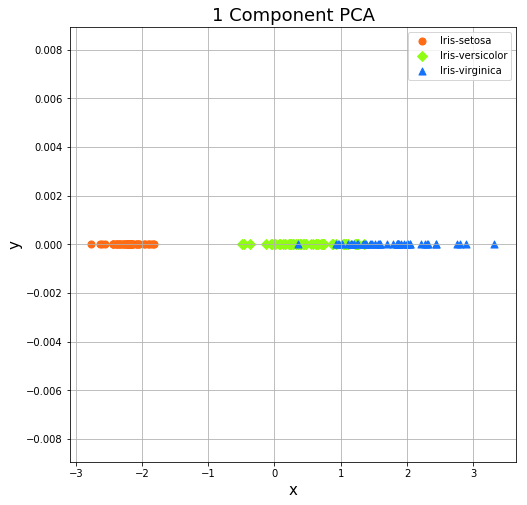
\includegraphics[width=0.3\textwidth]{lectDimRed/dimensionReduce_1d.png}
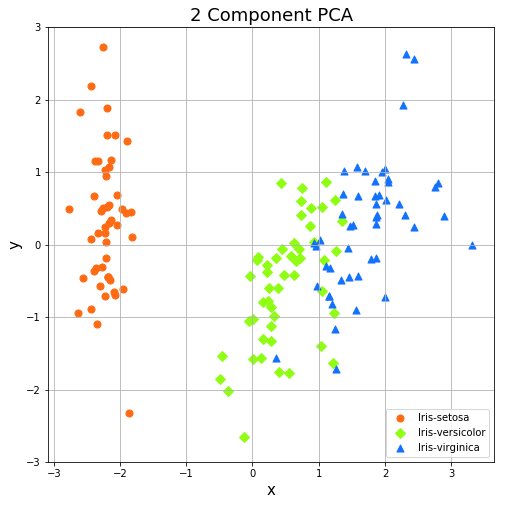
\includegraphics[width=0.3\textwidth]{lectDimRed/dimensionReduce_2d.png}
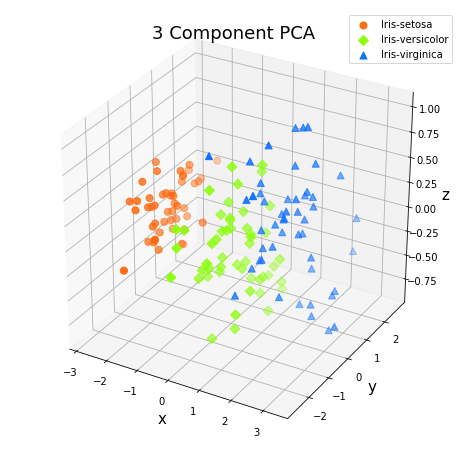
\includegraphics[width=0.3\textwidth]{lectDimRed/dimensionReduce_3d.png}
%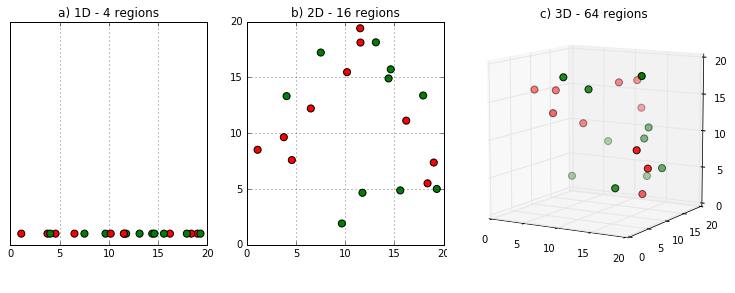
\includegraphics[width=0.6\textwidth]{lectDimRed/curse-dimensionality-2.png}\footnote{\url{www.kdnuggets.com/2017/04/must-know-curse-dimensionality.html}}
%\end{column}
%\end{columns}
%https://www.kdnuggets.com/2017/04/must-know-curse-dimensionality.html

\end{frame}
%***********************************************************
\begin{frame}{Dimensionality Reduction: Basic Idea}
\begin{itemize}
	\item Keep the dimensions that contain the most information
	\item Discard the least helpful dimensions
	\item Get the data down to a manageable size
	\item This is a type of feature extraction
\end{itemize}
	
\end{frame}
%***********************************************************
\begin{frame}{Dimensionality Reduction vs. Feature Selection}
\begin{itemize}
	\item Creates new, linear combinations of features vs. selecting subsets of features
	\item Built in attention to correlation
	\item New features may not be interpretable
\end{itemize}
	
\end{frame}


%***********************************************************
\begin{frame}{How to do Dimensionality Reduction}

\begin{columns}
\begin{column}{0.5\textwidth}
\begin{itemize}
\item Goal: Find the line(s) on which to project the data to show most of the variability
\item Approach: Compute a set of orthogonal (perpendicular) basis vectors
\item We do this by computing the Eigenvalues and Eigenvectors of the data
%
%\item Here, the first principle component has the most variance
%\item We want to compute
%\begin{enumerate}
%\item The direction of the tilt
%\item The extent of spread along each dimension
%\end{enumerate}
\end{itemize}
\end{column}
\begin{column}{0.5\textwidth}
\includegraphics[width=1\textwidth]{lectDimRed/Data2.pdf}
\end{column}
\end{columns}
\end{frame}

%***********************************************************
\begin{frame}{Eigenvalues and Eigenvectors}
\begin{columns}
\begin{column}{0.5\textwidth}
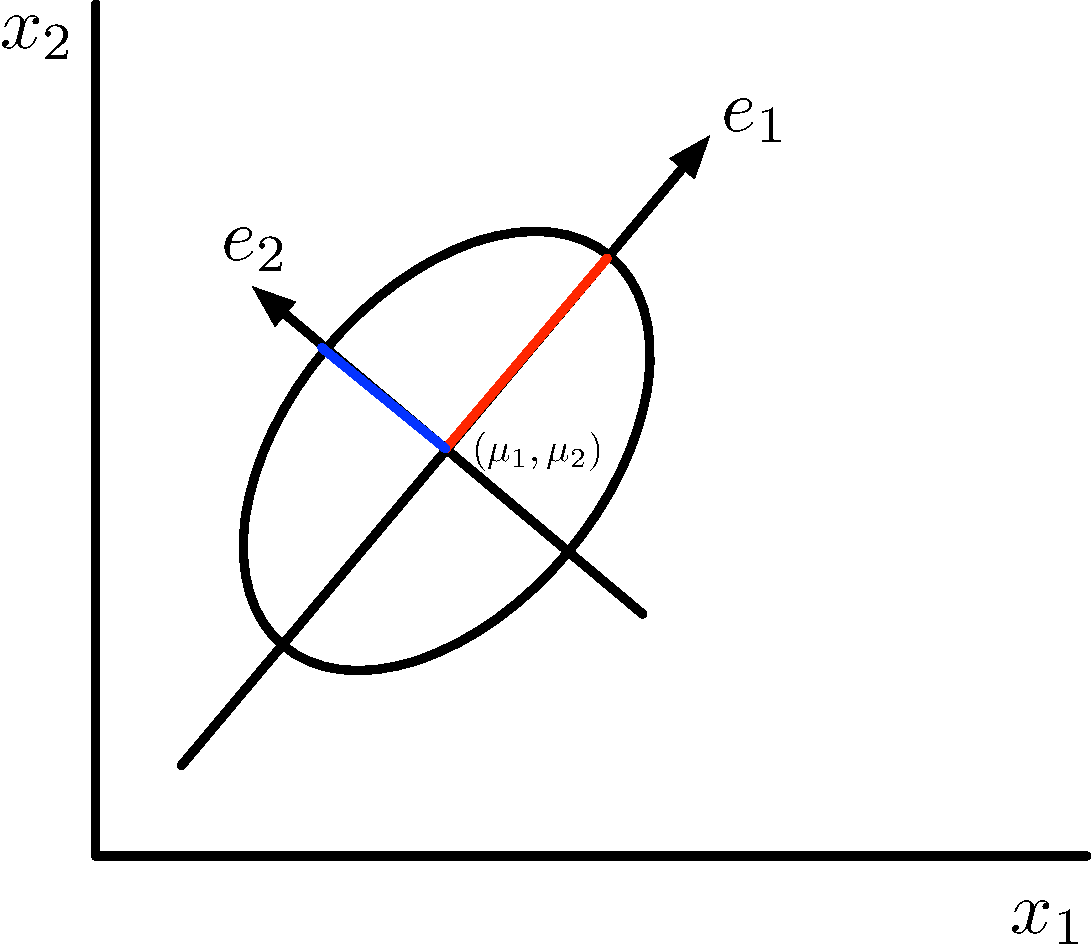
\includegraphics[width=1\textwidth]{lectDimRed/mvNormalv2.pdf}
\end{column}
\begin{column}{0.5\textwidth}
\begin{itemize}
\item The ellipse describes the shape of the data
\item The length of the red line is the value of the first Eigenvalue
\item The length of the blue line is the value of the second Eigenvalue
\item Each Eigenvector has direction based on the tilt of the data
\item  ...and the length is the Eigenvalue
%\item Center the data so \textbf{$\mu$}$ = 0$
% Eigenvector - typically normalized, just shows direction
\end{itemize}
\end{column}
\end{columns}

\end{frame}

%***********************************************************
\begin{frame}{What Does Our Data Look Like?}

\begin{columns}
\begin{column}{0.5\textwidth}
\begin{itemize}
\item $\textbf{X}$ is $n \times d$
\item $n \ll  d$
\begin{itemize}
\item Genomic data
\item Many more dimensions than data points
\item Each row is a patient
\item Each item is a feature: nucleotide, age, fasting blood glucose level, ...
\item Underconstrained / underspecified problem
\end{itemize}
\end{itemize}
\end{column}
\begin{column}{0.5\textwidth}
\begin{itemize}
\item $n \gg d$
\begin{itemize}
\item Netflix
\item Lots of users
\item Not so many movies
\item Not so many reviews
\item Not addressed by this approach
\item Overconstrained / overspecified problem 
\end{itemize}
\end{itemize}
\end{column}
\end{columns}
\[
\textbf{X}= n \overbrace{\begin{cases}
               \left[\begin{array}{ccccccc}
	x_{1,1} & x_{1,2} & \cdots& \cdots& \cdots& \cdots & x_{1,d}	\\
	x_{2,1} & x_{2,2} & \cdots & \cdots& \cdots& \cdots& x_{2,d}	\\
	\cdots & \cdots & \cdots & \cdots& \cdots& \cdots&\cdots	\\
	x_{n,1} & x_{n,2} & \cdots& \cdots& \cdots& \cdots & x_{n,d}	
\end{array}\right]
            \end{cases}}^d
\]
\end{frame}
%***********************************************************
\begin{frame}{Dimensionality Reduction}

\begin{itemize}
	\item \textbf{X} can be too big to operate on directly
	\item We want a linear transform to compute data matrix $\textbf{X}'$ with a reduced number of dimensions
\end{itemize}
%\begin{columns}
%\begin{column}{0.5\textwidth}
\[
X= n \overbrace{\begin{cases}
               \left[\begin{array}{cccccccccccccc}
	x_{1,1} & x_{1,2} & \cdots& \cdots& \cdots& \cdots& \cdots& \cdots& \cdots& \cdots& \cdots& \cdots& \cdots & x_{1,d}	\\
	x_{2,1} & x_{2,2} & \cdots & \cdots& \cdots& \cdots& \cdots& \cdots& \cdots& \cdots& \cdots& \cdots& \cdots& x_{2,d}	\\
	\cdots & \cdots & \cdots & \cdots& \cdots& \cdots& \cdots& \cdots& \cdots& \cdots& \cdots& \cdots& \cdots&\cdots	\\
	x_{n,1} & x_{n,2} & \cdots& \cdots& \cdots& \cdots& \cdots& \cdots& \cdots& \cdots& \cdots& \cdots& \cdots & x_{n,d}	
\end{array}\right]
            \end{cases}}^d
\]
%\end{column}
%\begin{column}{0.5\textwidth}
\[
X'= n \overbrace{\begin{cases}
               \left[\begin{array}{cccc}
	x'_{1,1} & x'_{1,2} & \cdots & x'_{1,m}	\\
	x'_{2,1} & x'_{2,2} & \cdots & x'_{2,m}	\\
	\cdots & \cdots & \cdots &\cdots	\\
	x'_{n,1} & x'_{n,2} & \cdots & x'_{n,m}	
\end{array}\right]
            \end{cases}}^m
\]
%\end{column}
%\end{columns}

\end{frame}
%***********************************************************
\begin{frame}{Computing \textbf{X}'}

\begin{itemize}
		\item Linear transform realized by a mapping matrix $\textbf{W}$ ($d$ rows, $m$ columns)
		\item So that $\textbf{X}' = \textbf{X} \textbf{W}$
\end{itemize}
\[
\begin{bmatrix} 
	 &   & 	\\
	 &   & 	\\
	 &   & 	\\
	 &   & 	\\
	 & \textbf{X}' & 	\\
	 &  & 	\\
	 &  & 	\\
	 & & 	\\
\end{bmatrix} 
= \begin{bmatrix} 
	&\hspace{12em}  & 	\\
	&  & 	\\
	&  & 	\\
	&  & 	\\
	&\textbf{X} & 	\\
	&  & 	\\
	&  & 	\\
	&  & 	\\
\end{bmatrix} 
\times
 \begin{bmatrix} 
	 &  \hspace{4em}& 	\\
	&  & 	\\
	  &  &\\
	  &  &\\
	  &  &\\
	  &  &\\
	  & \textbf{W} &\\
	  &  &\\
	  &  &\\
	  &  &\\
	  &  &\\
	  &  & 
\end{bmatrix} 
\]
\end{frame}

%***********************************************************
\begin{frame}{How Big are these Matrices?}

\begin{itemize}
\item $\textbf{X}'$ is $n \times m$
\item $m \ll d$
\item Recall $\textbf{X}' = \textbf{X} \textbf{W}$
\item Want to compute $\textbf{W}$ such that 
\item The columns of $\textbf{W}$ are the basis functions in the reduced space
\end{itemize}
\end{frame}
%***********************************************************
\begin{frame}{What can \textbf{W} do?}

\begin{itemize}
\item $\textbf{X}' = \textbf{X} \textbf{W}$
\item It can weight columns by zero
\item It can create new columns that are weighted sums of other columns
\item \ldots
\end{itemize}
\end{frame}
%***********************************************************
\begin{frame}{Classic Dimensionality Reduction Method: PCA}

\begin{itemize}
\item Basic idea: Compute a set of orthogonal (perpendicular) basis vectors
\item Then choose most important basis vectors (those with the most variance)
\item Those become the rows of the mapping matrix $\textbf{W}$
\item Then $\textbf{X} \textbf{W}$ projects down onto that basis, giving us \textbf{X$'$}
\end{itemize}
\begin{columns}
\begin{column}{0.5\textwidth}
\begin{itemize}
\item[?] If we want to draw a line that best describes the data, what line do we draw? % the first eigenvector
\end{itemize}
\end{column}
\begin{column}{0.5\textwidth}
\includegraphics[width=1\textwidth]{lectDimRed/Data2.pdf}
\end{column}
\end{columns}
\end{frame}
%***********************************************************
\begin{frame}{Classic Dimensionality Reduction Method: PCA}

\begin{itemize}
\item Basic idea: Compute a set of orthogonal (perpendicular) basis vectors
\item Then choose most important basis vectors (those with the most variance)
\item Those become the rows of the mapping matrix $\textbf{W}$
\item Then $\textbf{X} \textbf{W}$ projects down onto that basis, giving us \textbf{X$'$}
\end{itemize}
\begin{columns}
\begin{column}{0.5\textwidth}
\begin{itemize}
\item If we want to draw a line that best describes the data, what line do we draw? 
\item We draw the first Eigenvector
\end{itemize}
\end{column}
\begin{column}{0.5\textwidth}
\includegraphics[width=1\textwidth]{lectDimRed/Data2.pdf}
\end{column}
\end{columns}
\end{frame}
%***********************************************************
\begin{frame}{An Extreme Data Set}

\begin{columns}
\begin{column}{0.7\textwidth}
\begin{itemize}
\item Here there is no variability along the second dimension
\item In the extreme case, we could completely drop it
\item Note: When $d \gg n$ there will be some dimensions with Eigenvalue = 0  % basically, no variability in that dimension
\end{itemize}
\end{column}
\begin{column}{0.3\textwidth}
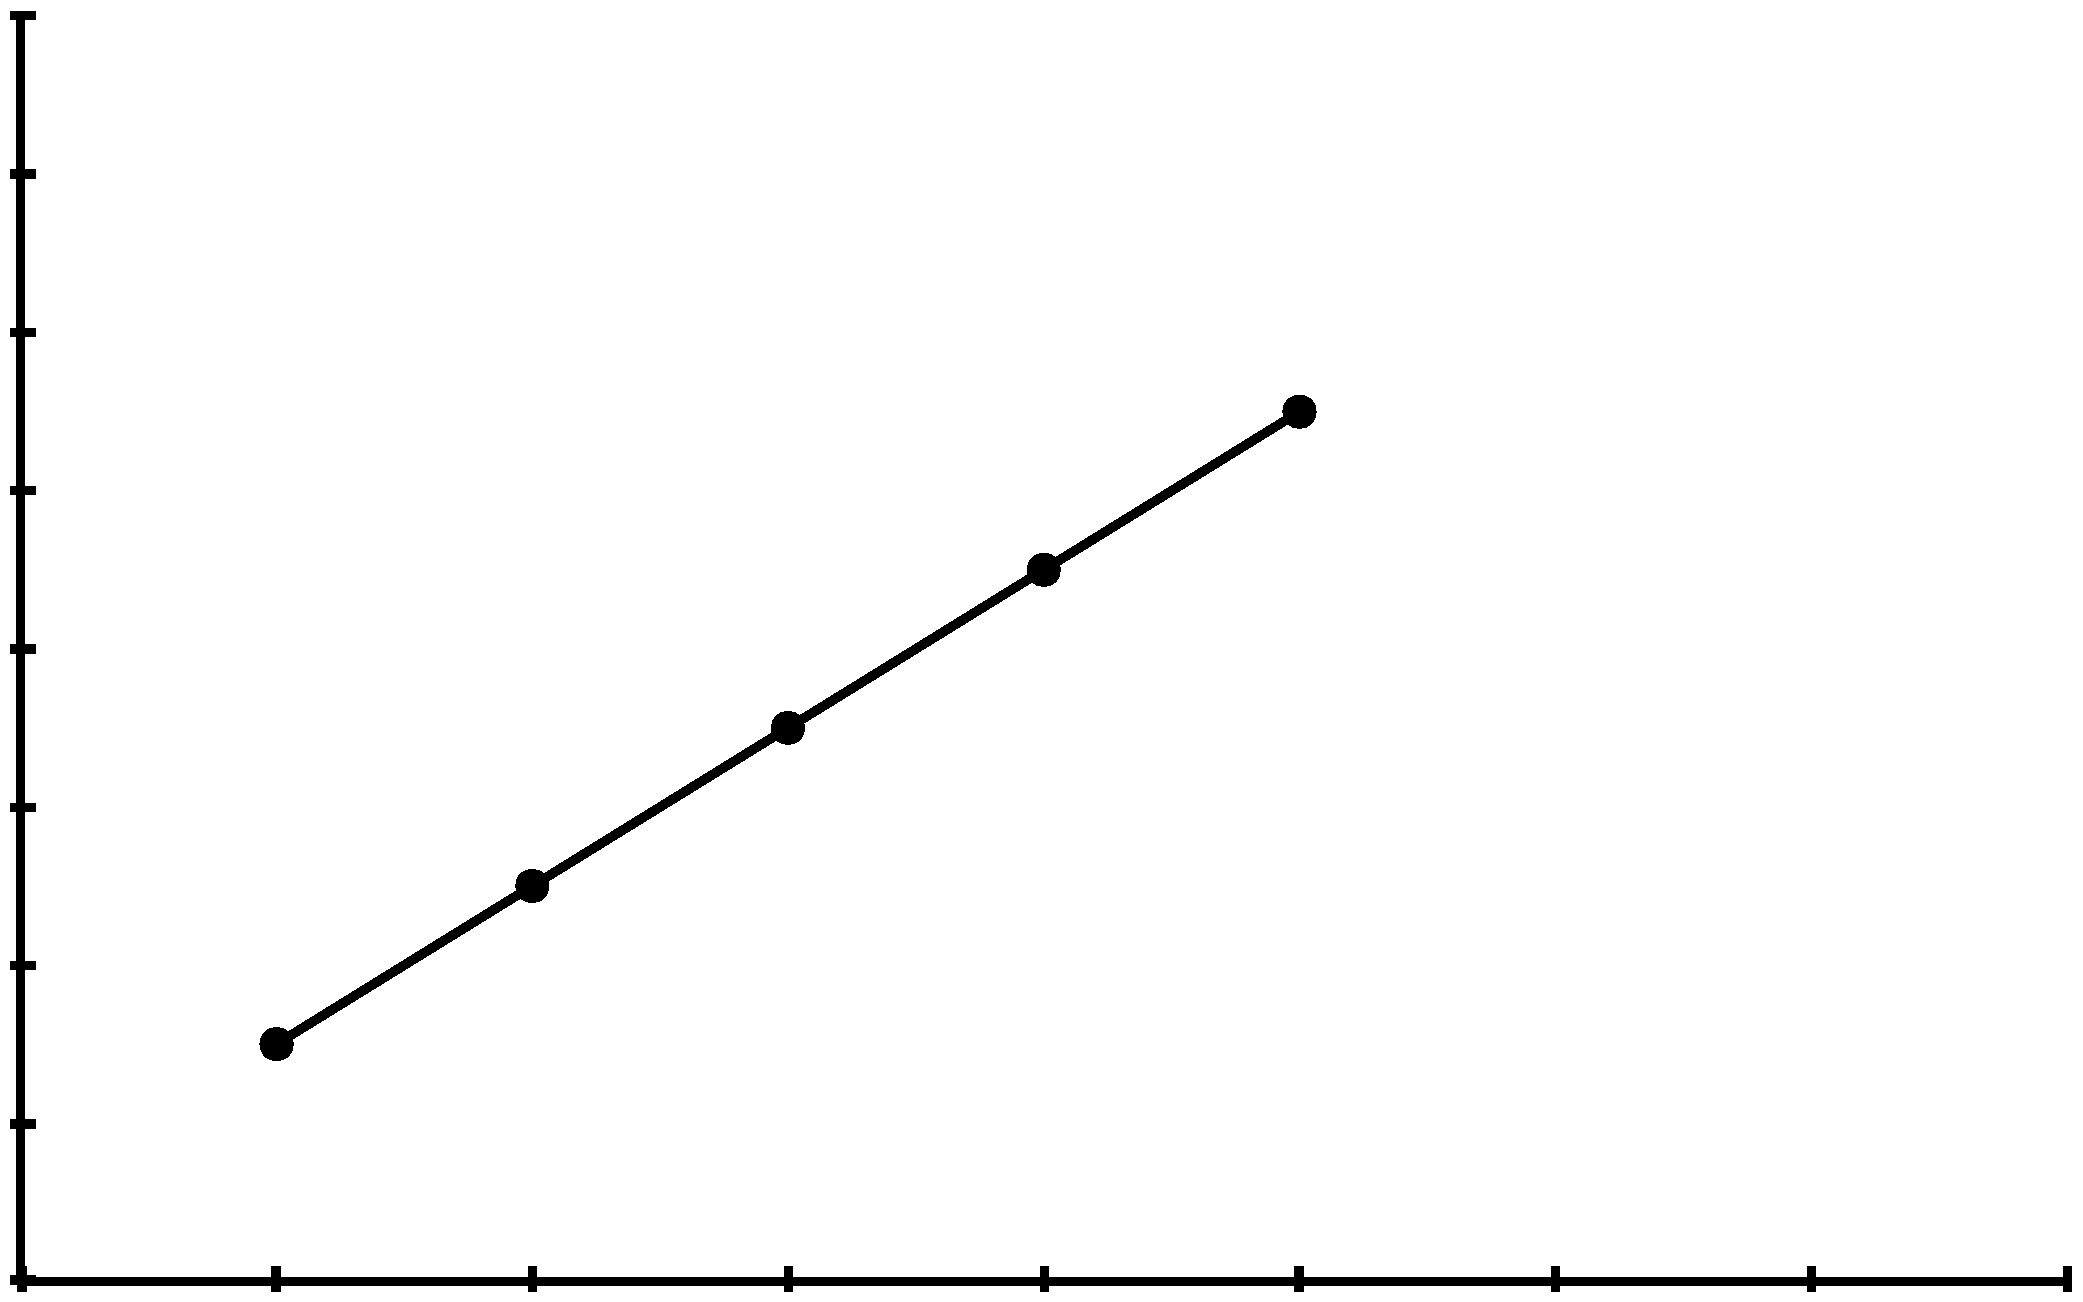
\includegraphics[width=1\textwidth]{lectDimRed/extremeMapping.pdf}
\end{column}
\end{columns}
\end{frame}
%***********************************************************
\begin{frame}{Classic Dimensionality Reduction Method: PCA}

\begin{itemize}
\item Principal Component Analysis
\item We want to lose the least amount of information
\item So we remove the dimensions with NO variability
\item Note that the number of principle components = the number of dimensions in our data
\item We want to drop out the low variance ones that aren't helpful
\item For example:
\begin{itemize}
\item If all of our data points are about people who are ages 18 - 19
\item ... or have a fasting blood glucose value in a very narrow, equivalent range
\item That piece of information is highly unlikely to be useful in discriminating between people
\end{itemize}
\end{itemize}
\end{frame}
%***********************************************************

\begin{frame}{Consider the Case of the  Multivariate Normal Distribution}
\begin{columns}[T]
\begin{column}{0.6\textwidth}
\begin{itemize}
	\item \textbf{Z} is an equation variable
	\item From the data matrix, \textbf{X} we get
	\begin{itemize}
		\item \textbf{$\mu$} is the vector of means, 1 for each dimension
		\item  $\Sigma$  is the covariance matrix of $\textbf{X}$
	\end{itemize}
	\item Each entry, $\sigma_{i,j} = E[(\textbf{X}_i - \mu_i)(\textbf{X}_j- \mu_j)]$
	\item $\Sigma$ is a symmetric matrix
	\item If $\Sigma$ is diagonal
	\begin{itemize}
		\item The dimensions of \textbf{X} are independent
	\end{itemize}
	%\item[?] Which features in this PDF matter the most / least?
	\item We leverage the covariance matrix to figure out which dimensions are most important
\end{itemize}
\end{column}
\begin{column}{0.4\textwidth}
\begin{itemize}
	\item[] 
	$$\textrm{pdf(\textbf{Z})} = \frac{exp^{(-\frac{1}{2}(\textbf{Z} - \pmb{\mu})^T\Sigma^{-1}(\textbf{Z} - \pmb{\mu}))}}{\sqrt{(2\pi)^k|\Sigma|}}$$	
\end{itemize}
\vspace{2em}
\[ \Sigma = 
%\begin{cases}
               \left[\begin{array}{cccc}
	\sigma_{1,1} & \sigma_{1,2} & \cdots & \sigma_{1,d}	\\
 	\sigma_{2,1} & \sigma_{2,2} & \cdots & \sigma_{2,d}	\\
	\cdots & \cdots & \cdots &\cdots	\\
	\sigma_{d,1} & \sigma_{d,2} & \cdots & \sigma_{d,d}	
\end{array}\right]
   %         \end{cases}
\]\end{column}
\end{columns}


\end{frame}
%***********************************************************
\begin{frame}{Consider the Case of the  Multivariate Normal Distribution}
\begin{itemize}

	\item From Linear Algebra, we know
\begin{itemize}
	\item The Eigenvectors of $\Sigma$ describe the direction of the spread in $\textbf{X}$
	\item The Eigenvalues of $\Sigma$ describe the magnitude of the Eigenvectors
	\item[] 
	\vspace{1em}
\item Now we know why we need them
\begin{itemize}
	\item To project data onto them to form the mapping matrix  $\textbf{W}$
\end{itemize}
\item We also know what they are
\begin{itemize}
	\item They determine the shape and spread of the data cloud
\end{itemize}
\item[?] How do we determine the Eigenvalues  \& Eigenvectors?
\end{itemize}
\end{itemize}

\end{frame}
%***********************************************************
\begin{frame}{How do we determine the Eigenvalues  \& Eigenvectors?}
\begin{enumerate}

\item Eigenvalue Decomposition
\item Singular Value Decomposition 
\end{enumerate}

\end{frame}
%***********************************************************
\begin{frame}{Computing the  Eigenvalues \& Eigenvectors}
% keep in mind - we are trying to find the most important relationships between the dimensions
% only works on square matrices, which the covariance matrix is
\begin{itemize}
	\item Method 1: EVD
	\item The covariance matrix \textbf{$\Sigma$} can be decomposed into \textbf{$\Sigma$} $= \textbf{V}\textbf{L}\textbf{V}^T$ % since the cov matrix is symmetric, we can use the transpose instead of the inverse
	\item This is the \textbf{Eigenvalue Decomposition} of \textbf{$\Sigma$}
	\item Where $\textbf{L}$ is a diagonal matrix of values, typically sorted in decreasing order, from left to right
	\item These values are called Eigenvalues
	\item The top left value is the largest / most significant
	\item The columns of $\textbf{V}$ are Eigenvectors
	\item ...and will be sorted by Eigenvalue magnitude
	\item Each Eigenvalue is how much variance exists across the Eigenvector
\end{itemize}
\end{frame}

%***********************************************************
\begin{frame}{Why  EVD Doesn't Work in High Dimensions}

\begin{itemize}
	\item It decomposes the covariance matrix $\Sigma$, which is $d \times d$, to get the Eigenvalues and Eigenvectors
	\item Recall that the $d \gg n$
		\item Computationally difficult
%		\item Ex: closed-form Linear Regression requires computing the inverse of the Gram matrix ($\textbf{X}^T{\textbf{X}}$)
		% also SVM kermel calculations
		\item The covariance matrix is $d \times d$, so taking the inverse is $O(d^3)$
		\item This can be done while $d < 50K$ or so
		\item Once the data gets ``big'' we can't use closed form approaches
\end{itemize}
\end{frame}
%***********************************************************
\begin{frame}{Why use the Covariance Matrix?}

\begin{itemize}
\item Because it's square
\item Because it describes the relationships between the different dimensions % this helps us determine what is most important
%\item Remember: We are looking for the most important ``dimensions''
\item It solves the Normal Equation from Linear Regression (closed form solution)
\begin{itemize}
\item $\textbf{X}r = b$
\item Where $r$ is the vector of regression coefficients
\item and $b$ is the vector of intercept terms
\item Note that we are not guaranteed to have a solution to this equation
\item Because the problem is underconstrained
\end{itemize}
\end{itemize}
\end{frame}
%***********************************************************
\begin{frame}{Why use the Covariance Matrix?}

\begin{columns}
\begin{column}{0.5\textwidth}
\begin{enumerate}
\item $\textbf{X}r = b$
\item $\textbf{X}^T\textbf{X}r = \textbf{X}^Tb$
\item $\frac{1}{n-1}\textbf{X}^T\textbf{X}r = \textbf{X}^Tb\frac{1}{n-1}$
\end{enumerate}
\end{column}
\begin{column}{0.5\textwidth}
\begin{enumerate}
\item Normal Equation
\item Multiply both sides by $\textbf{X}^T$
\item Multiply both sides 
\end{enumerate}
\end{column}
\end{columns}
\begin{itemize}
\vspace{1em}
\item Note that $\frac{1}{n-1}\textbf{X}^T\textbf{X}$ is the definition of a covariance matrix, \textbf{$\Sigma$} for data with mean 0
\item The $n-1$ term gives us a bias free estimator % from sample, subtract 1, since 1 fewer degrees of freedom because we know the variance
\end{itemize}
\end{frame}
%***********************************************************
\begin{frame}{Solve}


\begin{itemize}
\item[]  $\frac{1}{n-1}\textbf{X}^T\textbf{X}r = \textbf{X}^Tb\frac{1}{n-1}$
\item To solve for $r$, compute (\textbf{X}$^T$\textbf{X})$^{-1}$ % which is the inverse cov matrix in the pdf
 \item But this is very expensive to compute
 \item Instead we can approximate the calculation
 \item EVD gives the best approximation
 \item So, we do an EVD of $\Sigma$ to learn which dimensions are important
\end{itemize}
\end{frame}
%***********************************************************
\begin{frame}{Computational Complexity}

\begin{itemize}
\item Eigenvalue decomposition  is $O(d^3)$ 
\item Which leads us to Method 2:  Singular Value Decomposition (SVD) of $\textbf{X}$
\item In SVD, we operate on \textbf{X} directly, instead of $\Sigma$ because it is smaller
\item \textbf{X} is $n \times d$ and $\Sigma$ is $d\times d$
\item Recall $n \ll d$
\end{itemize}
\end{frame}
%***********************************************************
%\begin{frame}{Computing \textbf{X}'}
%
%\begin{itemize}
%		\item Linear transform realized by a mapping matrix $\textbf{W}$ ($d$ rows, $m$ columns)
%		\item So that $\textbf{X}' = \textbf{X} \textbf{W}$
%\end{itemize}
%\[
% \begin{bmatrix} 
%	 &  \hspace{4em}& 	\\
%	&  & 	\\
%	  &  &\\
%	  &  &\\
%	  &  &\\
%	  & \textbf{X}&\\
%	  &  &\\
%	  &  &\\
%	  &  & 
%\end{bmatrix} 
%\times
% \begin{bmatrix} 
%	&\hspace{12em}  & 	\\
%	&  & 	\\
%	&\textbf{X}^T & 	\\
%	&  & 	\\
%	&  & 	\\
%\end{bmatrix} 
%= \begin{bmatrix} 
%	 &  \hspace{11em}& 	\\
%	&  & 	\\
%	  &  &\\
%	  &  &\\
%	  & \textbf{$\Sigma$}&\\
%	  &  &\\
%	  &  &\\
%	  &  &\\
%	  &  &\\
%	  &  & 
%\end{bmatrix} \]
%\end{frame}
%
%
%***********************************************************
\begin{frame}{SVD Decomposition}

\begin{itemize}
	\item We want to avoid computing and using covariance matrix $\Sigma$  because it is \textbf{X}$^T$\textbf{X} and is of size $d \times d$
	\item[?] Can we get the Eigenvalues and Eigenvectors of $\Sigma$ by using \textbf{X} instead?
\end{itemize}
\end{frame}
%***********************************************************
\begin{frame}{SVD Decomposition}

\begin{itemize}
	\item We want to avoid computing and using covariance matrix $\Sigma$  because it is \textbf{X}$^T$\textbf{X} and is of size $d \times d$
	\item Can we get the Eigenvalues and Eigenvectors of $\Sigma$ by using \textbf{X} instead?
	\item The SVD of $\textbf{X} = \textbf{U} \textbf{S} \textbf{V}^T$
\begin{itemize}
	\item $\textbf{U}$ is a unitary matrix $(\textbf{UU}^T = 1)$
	\item $\textbf{V}$ is matrix of right singular vectors 
	\item \textbf{S} is a diagonal matrix of singular values
\end{itemize}
	\item Idea is that we can factorize $\textbf{X}$ instead of  \textbf{$\Sigma$}
	\item We can reduce the number of dimensions by projecting onto the space determined by the right singular vectors with the largest values 
	\item In this case, the biggest singular values correspond to the Eigenvalues with the largest magnitude % they could be negative
% right refers to V^T, left refers to U
\end{itemize}
\end{frame}
%***********************************************************
\begin{frame}{Using the SVD of \textbf{X}}

\begin{itemize}
	\item[]
	$\textbf{X} = \textbf{USV}^T$\\
\item[]
	$\textbf{X}^T\textbf{X} = (\textbf{VS}^T\textbf{U})(\textbf{USV}^T)$
\item[]
	$= \textbf{VS}^T\textbf{SV}^T$
	\item Where $ \textbf{S}^T\textbf{S}$ is \textbf{L} from EVD
	\item Where $\textbf{L}$ is a diagonal matrix of values, typically sorted in decreasing order, from left to right
	% Eigenvalues are always non-negative so, no ordering issues
\end{itemize}
\end{frame}
%***********************************************************
\begin{frame}{Dimensions \& Complexity, Revisited}

\begin{itemize}
\item  $\textbf{X}$ is $n \times d$
\item $\textbf{X}^T\textbf{X}$ is $d \times d$
\item When $d \gg n$
\item EVD is $O(d^3)$, operating on a $d \times d$ covariance matrix
\item SVD is $O(\min(d^2n, n^2d))$, because we are operating on $\textbf{X}$, instead of  $\textbf{$\Sigma$}$
\end{itemize}
\end{frame}


%%***********************************************************
%\begin{frame}{How to Handle?}
%
%\begin{itemize}
%	\item Deep Learning!
%	\begin{itemize}
%		\item Often better, but it's still a problem
%	\end{itemize}
%\end{itemize}
%\end{frame}
%***********************************************************
%\begin{frame}{How Else to Handle?}
%
%\begin{itemize}
%	\item Dimensionality reduction!
%	\item Recall we need to compute $\textbf{X}^T\Sigma\textbf{X}$ for the MV Normal case
%	\item MV normal pdf has $\Sigma^-1$ ???
%	\item If $\textbf{X}$ is really big, this is expensive and complex
%	\item General idea
%		\begin{itemize}
%		\item Let $\textbf{X}$ be data matrix ($n$ rows of data, $d$ columns of dimensions)
%		\end{itemize}
%	\item Want a linear transform to compute data matrix $\textbf{X}'$ in a reduced number of dimensions
%\end{itemize}
%\begin{columns}
%\begin{column}{0.5\textwidth}
%\[
%X= n \overbrace{\begin{cases}
%               \left[\begin{array}{ccccccc}
%	x_{1,1} & x_{1,2} & \cdots& \cdots& \cdots& \cdots & x_{1,d}	\\
%	x_{2,1} & x_{2,2} & \cdots & \cdots& \cdots& \cdots& x_{2,d}	\\
%	\cdots & \cdots & \cdots & \cdots& \cdots& \cdots&\cdots	\\
%	x_{n,1} & x_{n,2} & \cdots& \cdots& \cdots& \cdots & x_{n,d}	
%\end{array}\right]
%            \end{cases}}^d
%\]
%\end{column}
%\begin{column}{0.5\textwidth}
%\[
%X'= n \overbrace{\begin{cases}
%               \left[\begin{array}{cccc}
%	x'_{1,1} & x'_{1,2} & \cdots & x'_{1,m}	\\
%	x'_{2,1} & x'_{2,2} & \cdots & x'_{2,m}	\\
%	\cdots & \cdots & \cdots &\cdots	\\
%	x'_{n,1} & x'_{n,2} & \cdots & x'_{n,m}	
%\end{array}\right]
%            \end{cases}}^m
%\]
%\end{column}
%\end{columns}
%
%\end{frame}
%%***********************************************************
%\begin{frame}{Categorical Data}
%
%\begin{itemize}
%\item Caveat: Our data are not categorial
%\item Categorical data can be used, but this method doesn't work as well
%\end{itemize}
%\end{frame}
%
%%***********************************************************
%\begin{frame}{Our Goal}
%
%\begin{itemize}
%\item Reduce the dimensions of $\textbf{X}$ 
%\item By keeping the dimensions with the most variance
%\end{itemize}
%\end{frame}
%***********************************************************
\begin{frame}{How Do We Find the Dimensions with the Most Variance?}

\begin{itemize}
\item Options
\begin{enumerate}
\item Traditional approach: Eigenvalue Decomposition (EVD)
\item More efficient approach: Singular Value Decomposition (SVD)
\item Highly efficient approach: Random Matrix
\end{enumerate}
\item Taking into consideration
\begin{itemize}
\item $\textbf{X}$ is not square
\item So, it can't have Eigenvalues / Eigenvectors
\item So, we use the covariance matrix $\Sigma$ instead
\end{itemize}
\end{itemize}
\end{frame}

%***********************************************************
\begin{frame}{Which Dimensions Matter?}

\begin{itemize}
\item AKA How to Compute the Basis Vectors?
\end{itemize}
\begin{enumerate}
\item Center your data
\begin{itemize}
\item Subtract out the mean in each dimension
\item So the data has mean 0
\end{itemize}
\item Compute $\Sigma$
\item Do the EVD of $\Sigma =  \textbf{V}\textbf{L}\textbf{V}^T$
\begin{itemize}
\item Then the basis vectors are the Eigenvectors of data covariance matrix, $\Sigma$
 $$\Sigma = \frac{\textbf{X}^T\textbf{X}}{(n - 1)}$$
 \item Where $\Sigma$  is a $d \times d$ matrix
\end{itemize}
\item Get \textbf{W} from the vectors in \textbf{V}, using the largest values in \textbf{L}
\end{enumerate}
\end{frame}

%***********************************************************
\begin{frame}{How to Compute the Basis Vectors?}

\begin{itemize}

\item From the EVD of $\Sigma =  \textbf{V}\textbf{L}\textbf{V}^T$
\item Construct mapping matrix $\textbf{W}$ from the $m$ most important Eigenvectors
 \item That is, the leftmost columns of $\textbf{V}$ 
 \[
\begin{bmatrix} 
	 &   & 	\\
	 &   & 	\\
	 &   & 	\\
	 &   & 	\\
	 & \textbf{X}' & 	\\
	 &  & 	\\
	 &  & 	\\
	 & & 	\\
\end{bmatrix} 
= \begin{bmatrix} 
	&\hspace{12em}  & 	\\
	&  & 	\\
	&  & 	\\
	&  & 	\\
	&\textbf{X} & 	\\
	&  & 	\\
	&  & 	\\
	&  & 	\\
\end{bmatrix} 
\times
 \begin{bmatrix} 
	 &  \hspace{4em}& 	\\
	&  & 	\\
	  &  &\\
	  &  &\\
	  &  &\\
	  &  &\\
	  & \textbf{W} &\\
	  &  &\\
	  &  &\\
	  &  &\\
	  &  &\\
	  &  & 
\end{bmatrix} 
\]

\end{itemize}
\end{frame}
%***********************************************************
\begin{frame}{Dimensions}

\begin{itemize}
\item  $\textbf{X}$ is $n \times d$
\item $\textbf{X}^T\textbf{X}$ is $d \times d$
\item When $d \gg n$
\item EVD is $O(d^3)$, operating on a $d \times d$ covariance matrix
\item SVD is $O(\min(d^2n, n^2d))$, because we are operating on $\textbf{X}$, instead of  $\Sigma$
\end{itemize}
\end{frame}
%***********************************************************
\begin{frame}{How Many Eigenvectors to Use?}

\begin{itemize}
\item There's no magic number
\item Look at the values 
\item Decide how many you can handle, computationally
\item Red point is probably not a good choice to stop including Eigenvectors
\end{itemize}
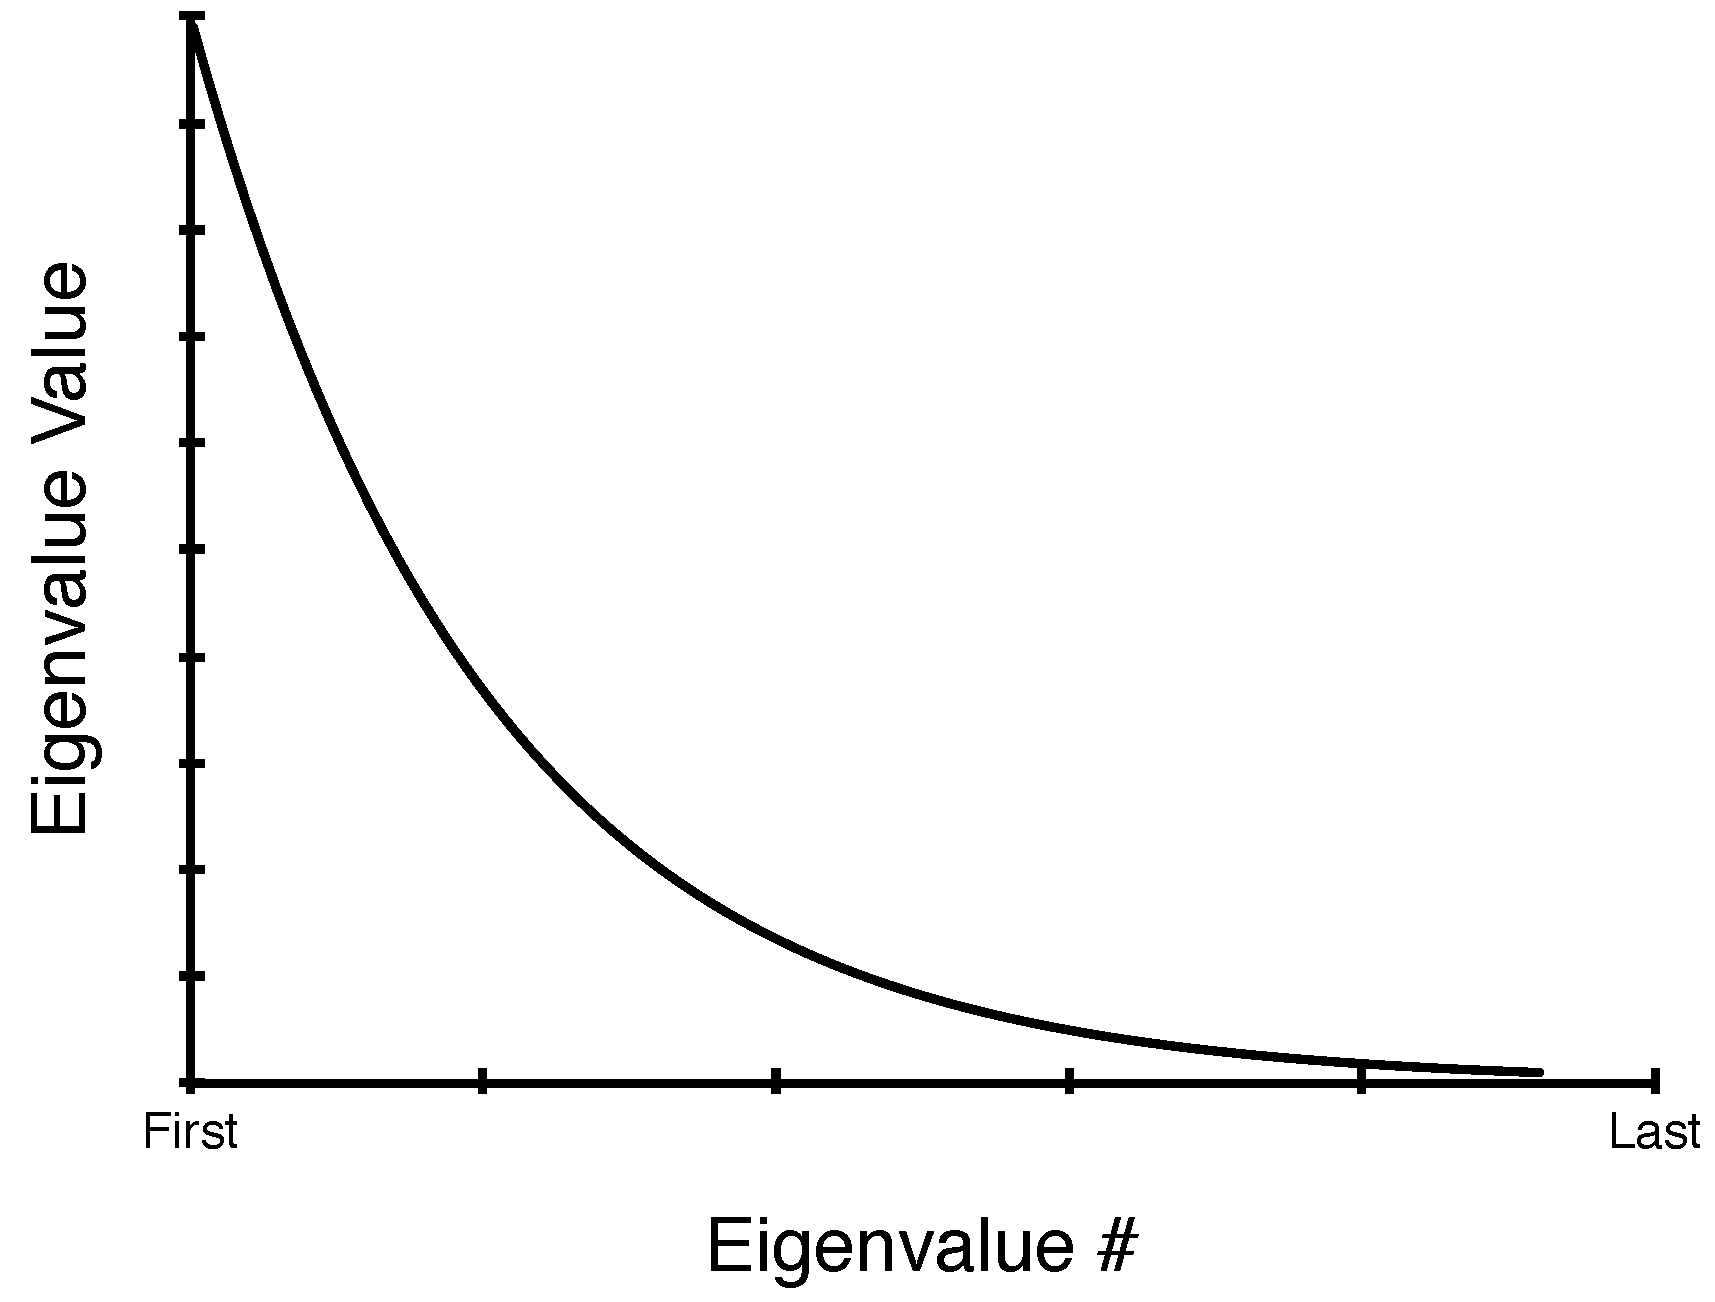
\includegraphics[width=.4\textwidth]{lectDimRed/eigenValues1.pdf} \hspace{5em}
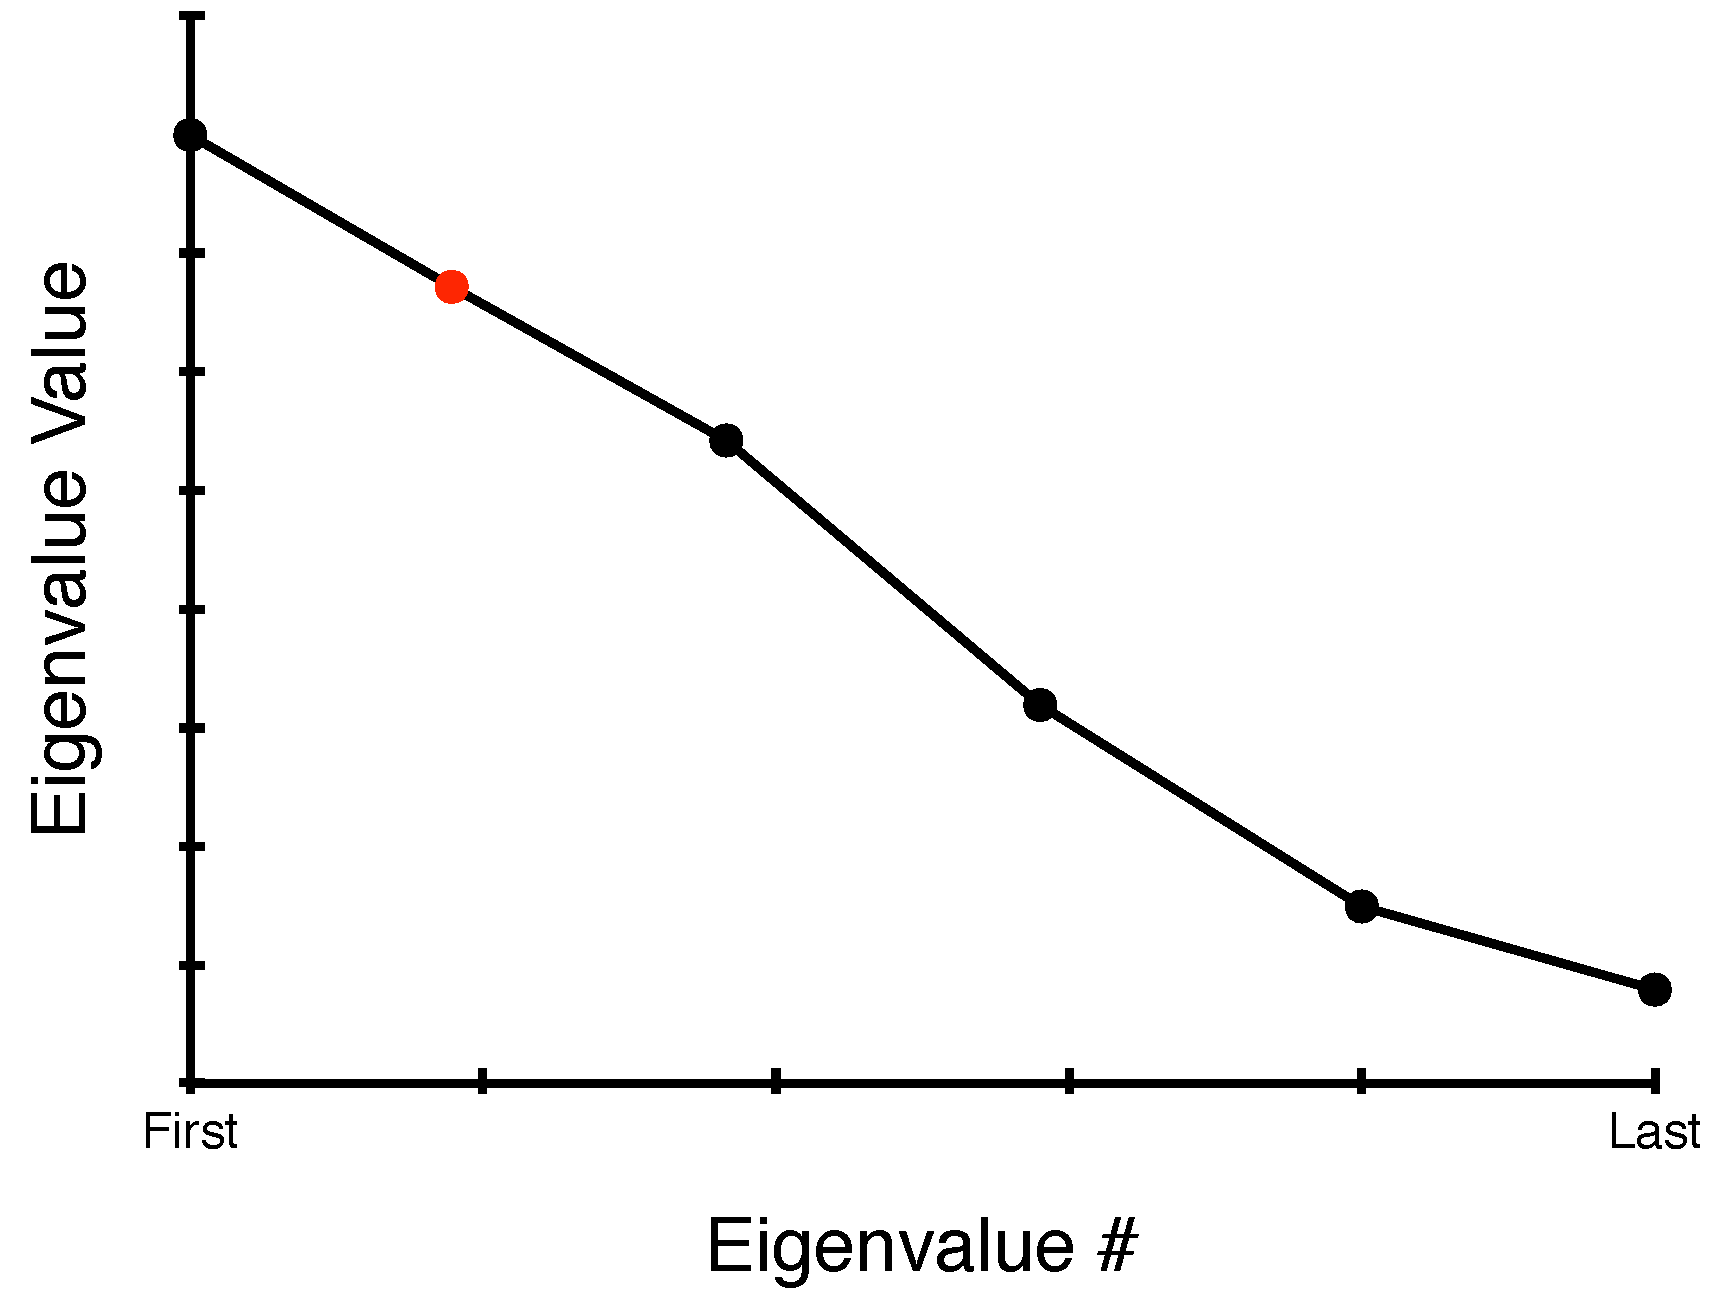
\includegraphics[width=.4\textwidth]{lectDimRed/eigenValues2.pdf}
\end{frame}
%***********************************************************
\begin{frame}{Even SVD Can Be Too Expensive}

\begin{itemize}
%\item SVD Complexity is $O(\min(d^2n, n^2d))$
\item In practice, just fill $\textbf{W}$ with samples from Normal$(0,1)$
	\begin{itemize}
	\item Known as a random projection\footnote{Bingham E, Mannila H, editors. Random projection in dimensionality reduction: applications to image and text data. Proceedings of the seventh ACM SIGKDD international conference on Knowledge discovery and data mining; 2001: ACM.}
	\item Often does a very nice job in practice!
	\item Johnson-Lindenstrauss Lemma
	\begin{itemize}
	\item Basic premise is that the distances between points in a high dimensional space are ``nearly preserved'' when they are projected on to a large enough random subspace
	% O(ndm) 
	
 	\end{itemize}

	\end{itemize}
\end{itemize}
\end{frame}
%***********************************************************
\begin{frame}{Summary Motivation}

\begin{itemize}
\item Why do it at all?
\begin{itemize}
\item Counteract the Curse of Dimensionality
\item Reduce computational burden
\end{itemize}
\end{itemize}
\end{frame}
%***********************************************************
\begin{frame}{Summary of Methods}

\begin{itemize}
\item PCA via Eigenvalue decomposition
\begin{itemize}
\item Classic approach
\item Can be difficult for even good software to do the math correctly (consider ill-conditioned matrices)
\end{itemize}
\item  PCA via SVD 
\begin{itemize}
\item Avoids the covariance matrix entirely, we operate directly on \textbf{X}
\item Considered more stable numerically
\item Computationally faster
\item But still very expensive
\item Results in the same \textbf{W}
\end{itemize}
\item Random Projections
\begin{itemize}
\item Not as precise
\item May not get the dimensions with the most variance
\item But is computationally feasible
\end{itemize}
\end{itemize}
\end{frame}
%***********************************************************

\begin{frame}{Questions?}
\begin{itemize}
	\item What do we know now that we didn't know before?
\begin{itemize}
	\item We know what the curse of dimensionality is and why it is a problem
	\item We know that it's possible to reduce the dimensions of our data
	\item We know some approaches to perform dimensionality reduction
	\item We know some trade-offs between the approaches
\end{itemize}

	\item How can we use what we learned today?
\begin{itemize}
	\item We can choose an appropriate method for dimensionality reduction
	\end{itemize}
\end{itemize}
\end{frame}


\end{document}

